\newpage
\subsection{Grenzfrequenz des Hochpasses}\label{sec:2-2}

\begin{highlightblock}[Grenzfrequenz des Hochpasses der AC-Kopplung]
	Es soll ermittelt werden, welche Grenzfrequenz der Hochpass der AC-Kopplung des
	Oszilloskops aufweist. Hierzu gibt es zwei Methoden, die im Versuchsaufbau beschrieben
	werden. Im Anschluss kann die Kapazität des Koppelkondensators berechnet werden.
	\begin{enumerate}[label=\textbf{\alph*:}, ref=\alph*, noitemsep]
		\item\label{itm:2-P2-1} Methode A: Speisung mit einer Sinusspannung variabler Frequenz.
		\item\label{itm:2-P2-2} Methode B: Speisung mit einem niederfrequenten Rechtecksignal.
		\item\label{itm:2-P2-3} Berechnung der Kapazität $C_\mathrm{AC}$ des Koppelkondensators.
	\end{enumerate}
\end{highlightblock}

\subsubsection{Verwendetes Material}

\begin{table}[h]
	\centering
	\caption{Verwendetes Material}
	\begin{tabularx}{\textwidth}{XXX}
		\textbf{Messgerät} & \textbf{Verwendung} & \textbf{Anmerkungen}\\ \midrule
		TDS2014C & Oszilloskop & \\
		Agilent 33250A & Funktionsgenerator & \\
	\end{tabularx}	
\end{table}

\subsubsection{Versuchsaufbau}

\marginref{\ref{itm:2-P2-1}}

Bei der ersten Methode macht man sich zunutze, dass die Amplitude eines
Sinussignals bei der 3dB-Grenzfrequenz auf $\frac{1}{\sqrt{2}}$ des
ursprünglichen Wertes abgefallen ist. Am Funktionsgenerator wird eine
Sinusspannung mit $\SI{5}{\volt}_{PP}$ Amplitude und variabler Frequenz
eingestellt.

Sobald die Frequenz so weit erhöht wurde, dass die Amplitude auf
$\frac{1}{\sqrt{2}}\cdot\SI{5}{\volt}_{PP} \approx \SI{3.54}{\volt}_{PP}$
abgefallen ist, wird die Frequenz abgelesen. Diese entspricht der Grenzfrequenz
$f_g$ des Hochpasses. Wie man im \autoref{fig:21-3db-grenzfrequenz} sieht,
liegt die Grenzfrequenz bei $\SI{7}{\hertz}$.

\begin{figure}[h]
	\centering
	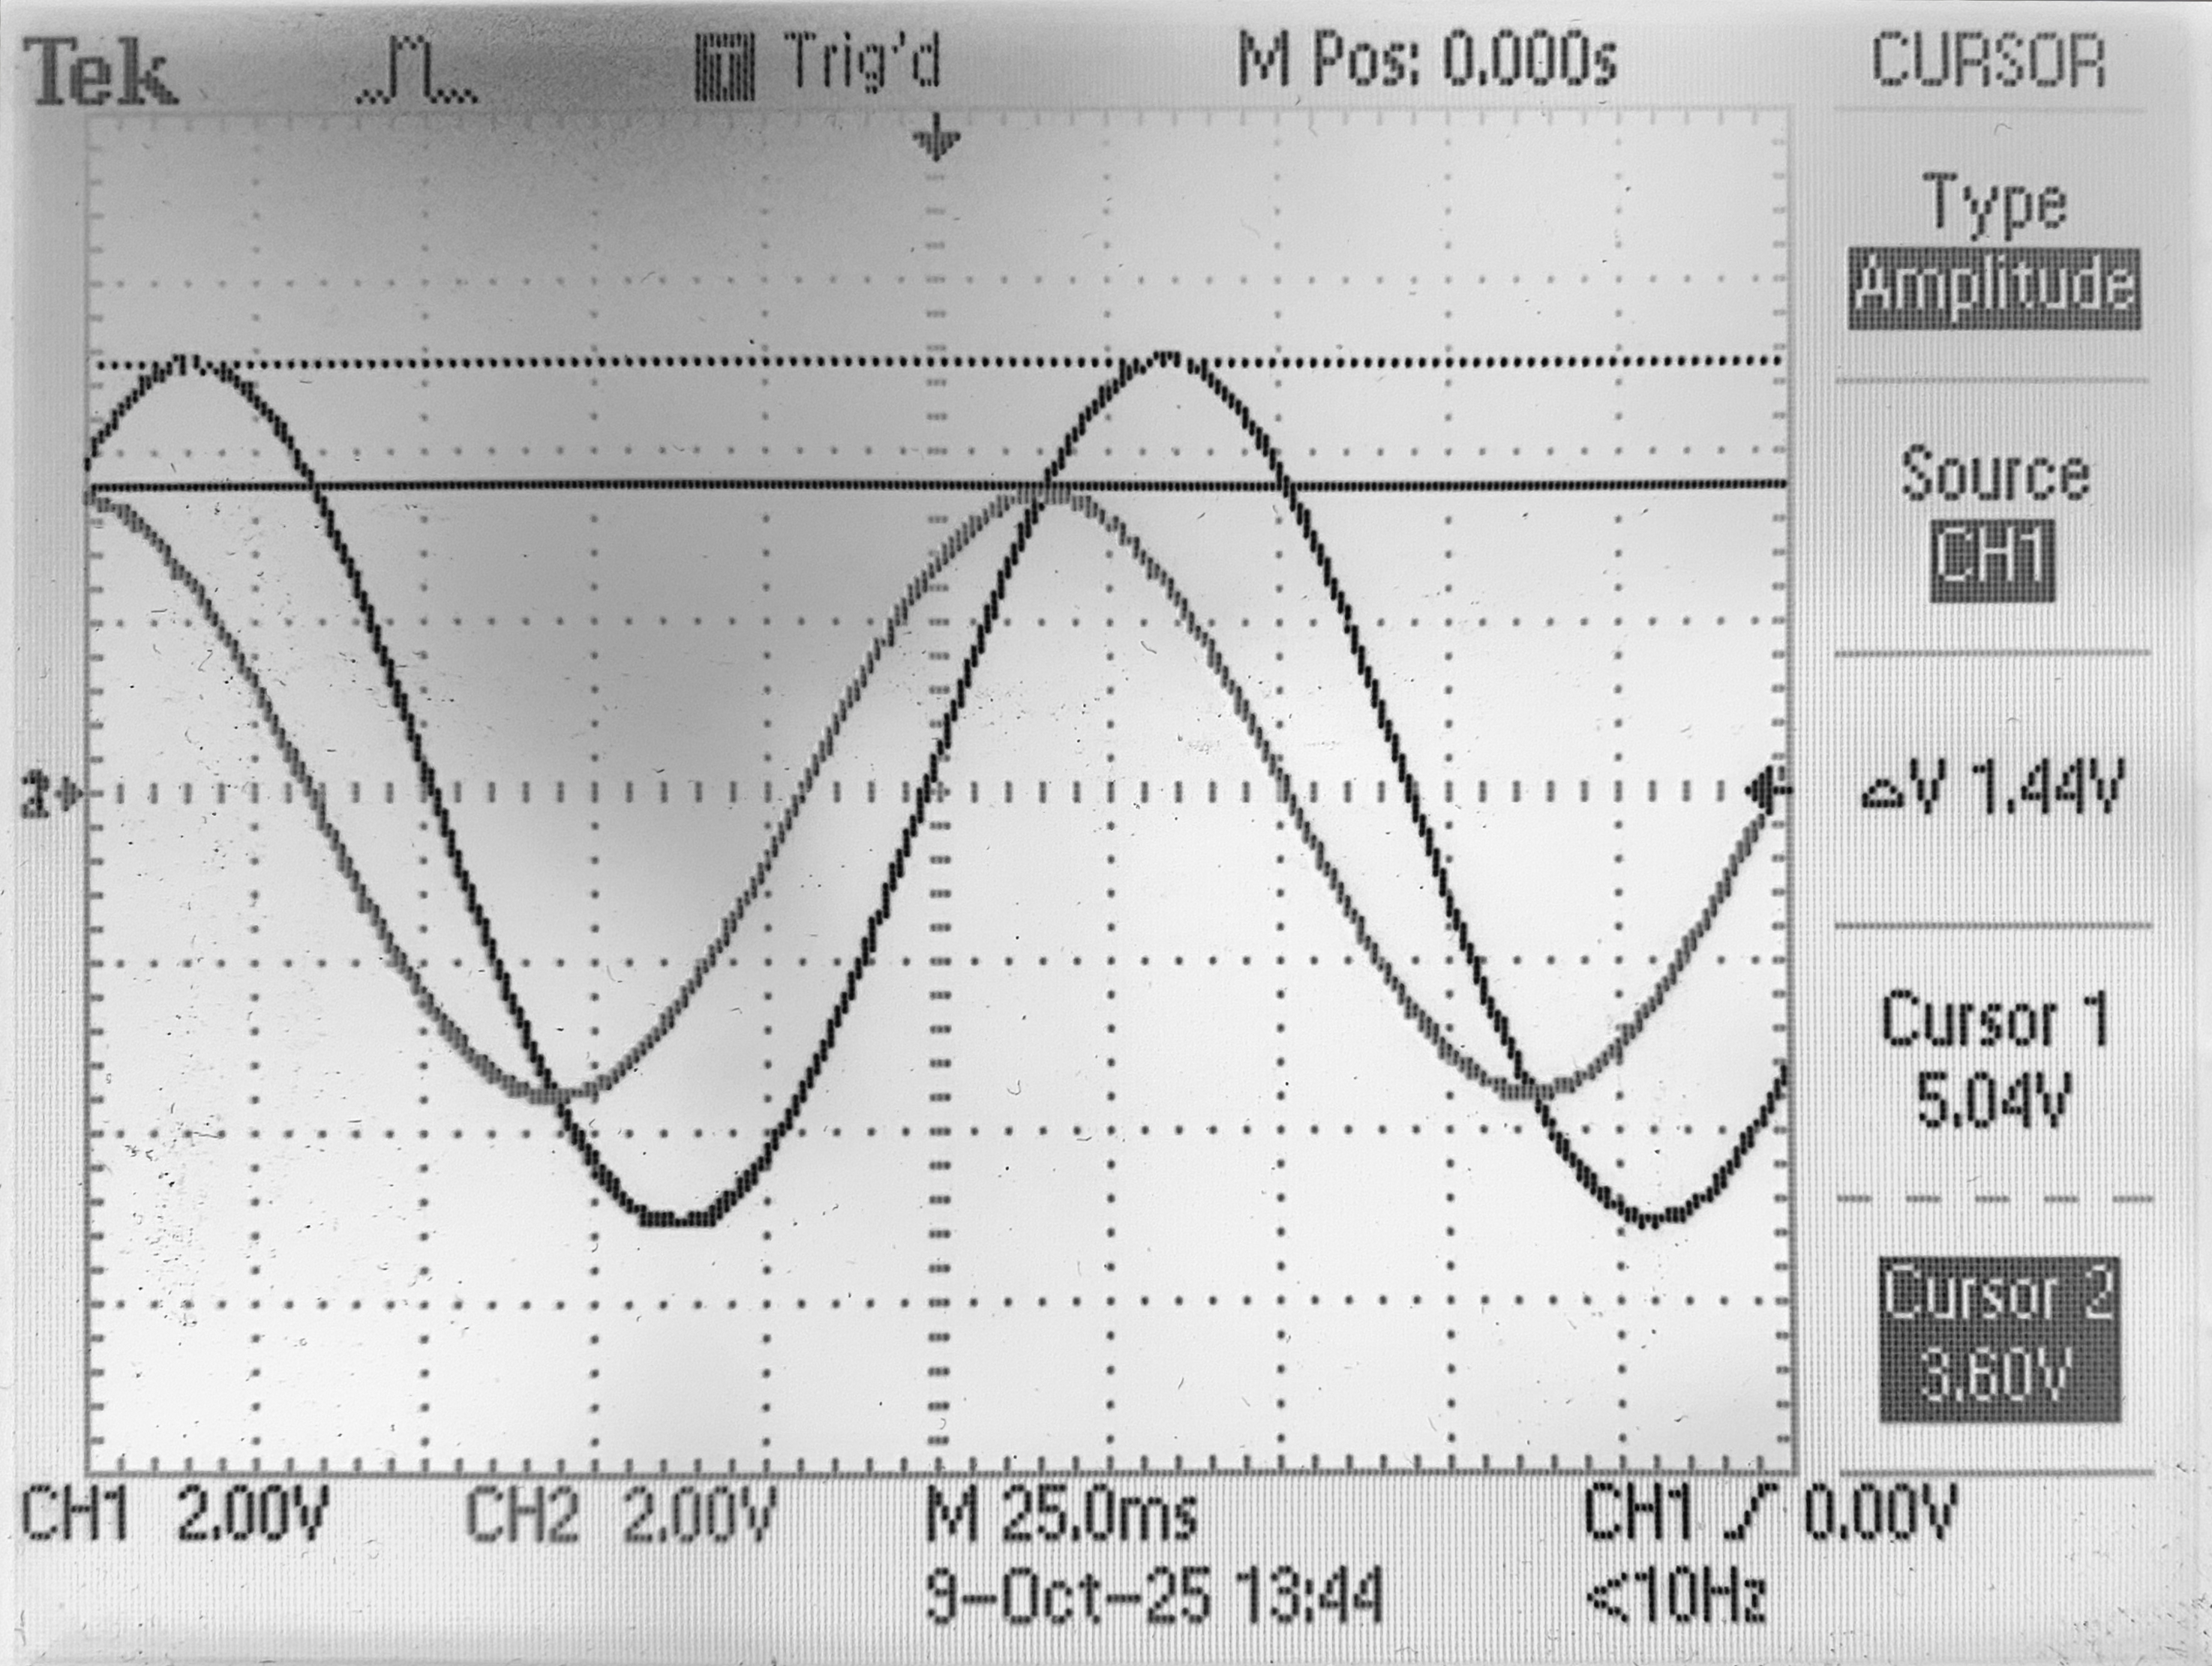
\includegraphics[width=7cm]{images/22_C-AC_Methode1.JPEG}
	\caption{Oszillogramm mit der 3dB Grenzfrequenz}
	\label{fig:21-3db-grenzfrequenz}
\end{figure}

\marginref{\ref{itm:2-P2-2}}

\begin{figure}[h]
	\centering
	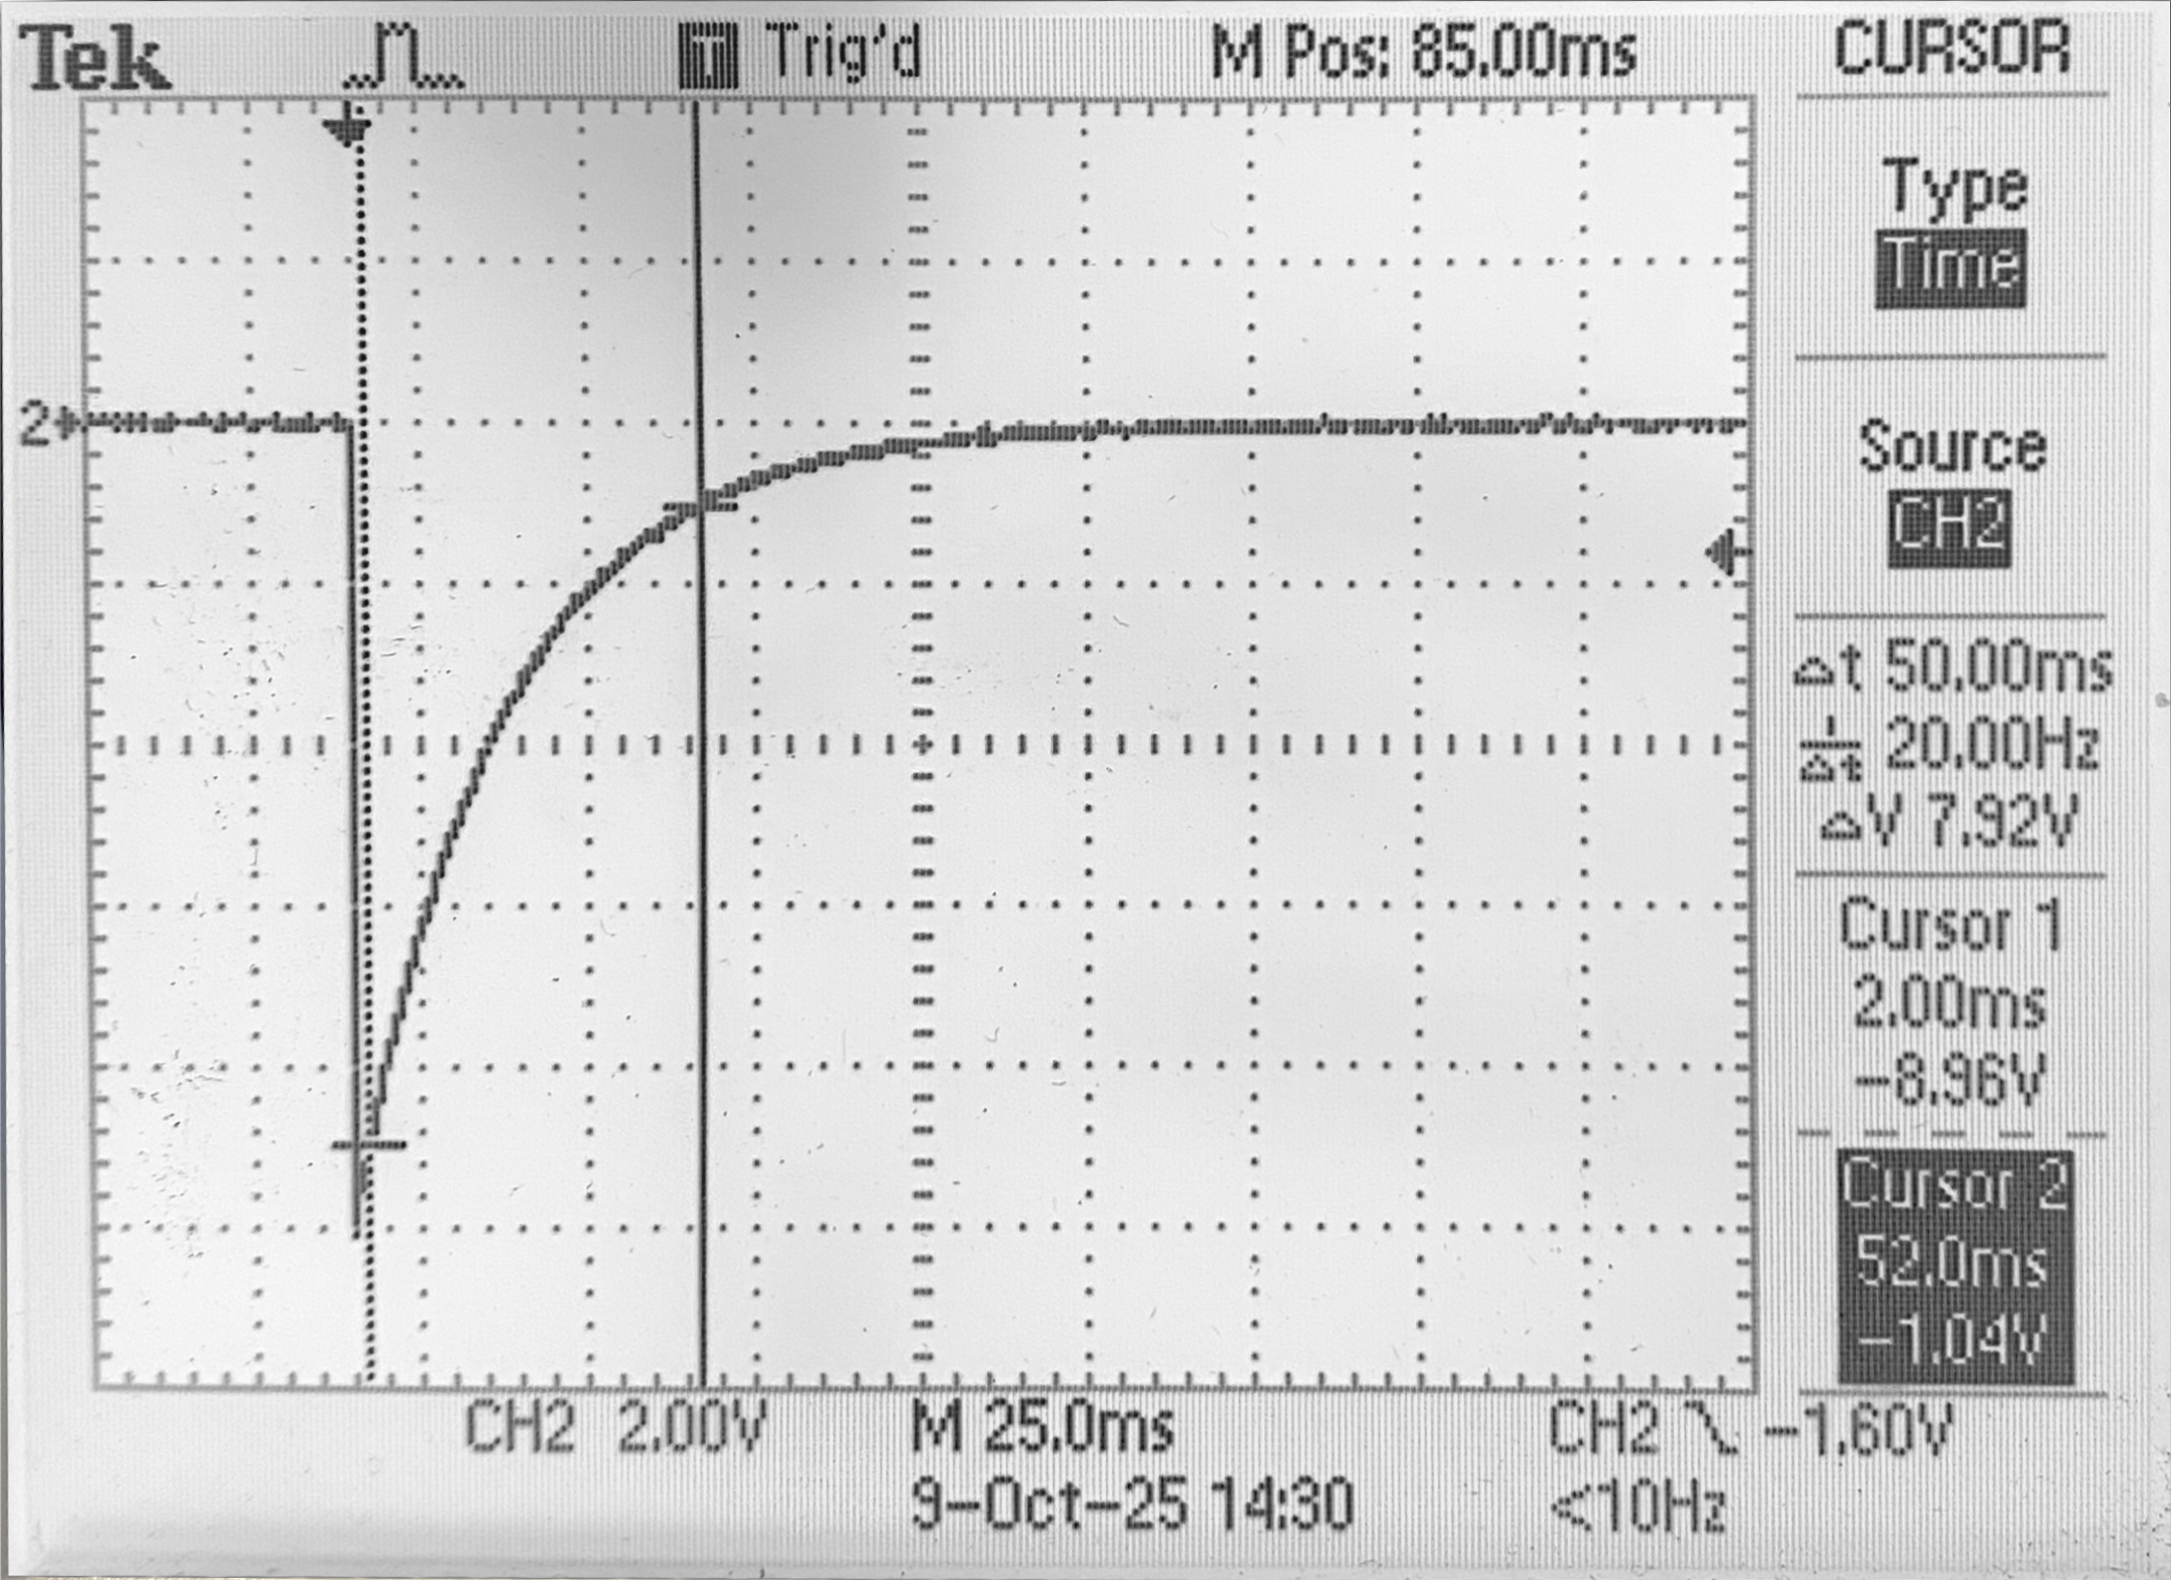
\includegraphics[width=7cm]{images/22_C-AC_Methode2.JPEG}
	\caption{Oszillogramm mit 10\%-90\% Anstiegszeit}
	\label{fig:21-10-90-anstiegszeit}
\end{figure}


\marginref{\ref{itm:2-P2-3}}

\subsubsection{Erkenntnisse}